% ML4PS 2026 (NeurIPS "Machine Learning and the Physical Sciences"), 11 Dec 2026, Atlanta.
% Deadline 12 Sep 2026, 23:59 AoE.
%
% GUIDELINES (retrieved 2026-08-22, all desk-reject material):
%   * NeurIPS 2026 template, UNMODIFIED. This file is still plain article class and must be
%     ported. Everything below is written to survive that port unchanged.
%   * Footer must read: "Submitted to the 9th Workshop on Machine Learning and the Physical
%     Sciences (ML4PS 2026). Do not distribute."
%   * DOUBLE-BLIND, fully anonymized -- "code, links, and all text and figures". No
%     institution name appears below; the artifact link needs an anonymized mirror.
%   * 4 pages excluding references. Appendices discouraged and unread, so nothing
%     load-bearing may live in one.
%
% FRAMING (PLAN.md Part II): ML4PS took 2 medical-imaging papers in 2024 and zero in 2025,
% and the committee is HEP / astro / simulation-based inference. This reads as an
% inverse-problems paper that happens to use MRI. "Prostate" appears twice.
%
% RE-SPINED 2026-08-22. The old spine was the synthetic inverted-U (C5). It is now a
% supporting result: the real-arm test that was meant to carry it has leverage for one
% parameter of four (RESULTS.md Phase 4). The spine is C23/C24, which is measured on 4,608
% exams and holds identically on five instruments.
%
% Every \todo marks something unwritten or unmeasured. Every number traces to paper/CLAIMS.md.
\documentclass{article}

% NeurIPS 2026 style, UNMODIFIED, as the guidelines require. `dblblindworkshop` routes the
% workshop title into the footer and, on its own, keeps the author block anonymous. `final`
% is what deanonymises: it sets \@anonymousfalse and replaces the submission footer
% ("Submitted to ... Do not distribute.") with the workshop track line. Drop `final` to get
% the submission form back.
\usepackage[dblblindworkshop,final]{neurips_2026}
\workshoptitle{Machine Learning and the Physical Sciences}

% The workshop mandates an exact footer string that differs from the style file's default
% ("Submitted to 40th Conference on Neural Information Processing Systems..."). This overrides
% it from the DOCUMENT, which leaves neurips_2026.sty untouched -- the guidelines prohibit
% modifying the template, and they also require this string, so it has to be done here.
% The string below is the one the CFP mandates for SUBMISSION. Under `final` it would be
% wrong on a published paper, so the override is skipped and the template's own workshop
% track line is used instead.
\makeatletter
\if@neuripsfinal\else
  \renewcommand{\@noticestring}{%
    Submitted to the 9th Workshop on Machine Learning and the Physical Sciences (ML4PS 2026).
    Do not distribute.%
  }
\fi
\makeatother

\usepackage{amsmath,amssymb,booktabs,graphicx,xcolor}
\usepackage{url}
% DRAFT SWITCH. \claim cross-references CLAIMS.md and \todo marks unfinished work; both are
% internal bookkeeping and neither belongs in a submitted PDF. Uncomment the next line to see
% them while writing. OFF by default, so the file cannot be compiled and sent with
% "[C23, C24]" scattered through the prose -- which is what happened once.
% \def\showdraftmarks{}
\ifdefined\showdraftmarks
  \newcommand{\todo}[1]{\textcolor{red}{[TODO: #1]}}
  \newcommand{\claim}[1]{\textcolor{blue}{\footnotesize[#1]}}
\else
  % \unskip removes the space that precedes the macro. Without it every "... \claim{C12}."
  % compiles to "... ." -- 18 of them, visible in the PDF as a gap before the full stop.
  \newcommand{\todo}[1]{\unskip}
  \newcommand{\claim}[1]{\unskip}
\fi

\title{Fisher information over-predicts how much of a\\
fitted MRI parameter comes from the prior}
% DOUBLE-BLIND: author block stays commented until camera-ready.
\author{%
  Kaushik Madapati\thanks{Also at College of Engineering, University of California, Berkeley.},
  \ Jie Bao, \ Yang Yang, \ Kang Wang, \ Hanxue Gu \\
  University of California, San Francisco
}
\date{}

\begin{document}
\maketitle

\begin{abstract}
Physics-based inverse models use prior assumptions to resolve parameters that the measurements
cannot uniquely determine, so understanding how strongly those assumptions influence an estimate is
essential for interpreting the physical quantities recovered. We investigate whether Fisher
information accurately predicts that influence in nonlinear quantitative MRI. Perturbing the prior
mean and refitting identical measurements gives a direct measurement of the sensitivity of maximum
a posteriori estimates. Across 4{,}608 clinical prostate exams from five scanner models, median
responses to prior shifts are roughly one-third smaller than Fisher-based predictions. We trace the
discrepancy to a residual-dependent curvature term that is small in overall magnitude but
consequential along poorly constrained parameter directions. Including it substantially improves
agreement between predicted and measured responses at the cohort level. These findings identify a
failure mode of Fisher-based sensitivity analysis: a small curvature error can produce a large
error in estimated prior dependence when the inverse problem is underdetermined.
\end{abstract}

%======================================================================
\section{Introduction}

A quantitative MRI exam measures a handful of images and infers tissue parameters from them by
inverting a known signal model. The parameters are meant to be properties of the tissue: two
scanners imaging the same patient should report the same $T_2$, where the raw images they produce
would differ. This is the premise of the harmonization literature, and of every method that
recovers physical parameters from a forward model \cite{borges2023,phycharm2025,vanlune2026,qiu2023,bloch_pinn2023}.

However, the inversion is ill-posed. A routine prostate exam provides three measurements per
voxel: a $T_2$-weighted image, a diffusion-weighted image (DWI), and an apparent diffusion
coefficient (ADC) map. Against these stand four unknowns: proton density (PD), the relaxation times $T_1$ and
$T_2$, and the diffusion coefficient $D$. The data alone therefore cannot determine them. To close the fit, every method adds a prior: a penalty pulling each estimate toward a
nominal tissue value, or, in a learned method, a training population that exerts the same pull
without being written down. Whatever the images do not determine, the prior determines instead. An
estimate is therefore part measurement and part prior, and how the two divide depends on the
acquisition, which differs between scanners.

Fisher information is the standard tool for reasoning about the first part: the matrix says how
much an acquisition carries about each parameter, and the Cram\'er--Rao bound built from it gives
the lowest variance any unbiased estimator can achieve. This literature already uses it: Zhang
et al.\ weight a network's training loss by that bound and verify the trained network approaches
it \cite{zhang2022}. That is, however, a statement about \emph{variance}, and even there the
matrix is known to mislead outside the high-signal regime \cite{vallisneri2008}. The same matrix
makes a second prediction, about \emph{bias}: how far the prior pulls each estimate from the value
the data alone would give. That one is rarely tested. We test it here, and it is wrong
by a consistent, reproducible amount.

\medskip\noindent\textbf{Contributions.}\footnote{Code, tests and the analysis arms:
\url{https://github.com/kaushikmadapati7/fisher-prior-sensitivity}. The clinical images are
not redistributable, so the cohort runs cannot be reproduced from it; everything that does not need
them can be.} We measure the prior's contribution to a fitted parameter
directly, by shifting the prior and observing how far the fit follows, rather than inferring it
from a bound. We compare that measurement against the Fisher prediction on 4{,}608 clinical exams
and five scanner models. We trace the discrepancy to a curvature term whose omission from the
Fisher matrix is standard, and show why the usual argument for omitting it does not hold when the
matrix is nearly singular.

%======================================================================
\section{Methods}

\paragraph{Signal model and notation.} For one voxel, write the four unknown tissue parameters as
a vector $x$, holding the logarithms of proton density (PD), $T_1$, $T_2$ and the diffusion
coefficient $D$. Working in
logarithms keeps every parameter positive and makes the prior scale-free. A clinical prostate exam
supplies three measurements of that voxel, whose logarithms form the vector $y$: a
$T_2$-weighted image, a DWI, and an ADC map. Three measurements stand against four unknowns. The
signal model $f$ predicts $y$ from $x$ given the acquisition settings recorded in the DICOM header
of every exam, namely repetition time (TR), echo time (TE) and $b$-value:
\begin{equation*}
  y = f(x) + \varepsilon ,
\end{equation*}
with $\varepsilon$ the measurement noise.

\paragraph{The estimator and the prior.} We estimate $x$ by maximum a posteriori (MAP) fitting:
the value that best explains the images subject to a Gaussian prior of mean $x_0$ and precision
$\Lambda = I / \sigma_{\text{prior}}^2$. The mean holds nominal prostate tissue values, PD $0.6$,
$T_1$ $1400$\,ms, $T_2$ $80$\,ms and $D$ $1.3\times10^{-3}$\,mm\textsuperscript{2}/s, the last
measured from this cohort. We set $\sigma_{\text{prior}} = 10$ in log units, which is a very weak
prior; Section~3 shows the result is insensitive to it over two decades \claim{C48}. Write $J = \partial f/\partial x$
for the Jacobian, the $3 \times 4$ matrix whose entries say how strongly each measurement responds
to each parameter, and $W$ for the inverse noise covariance, the diagonal matrix that weights a measurement by how
precise it is. We take $W = \sigma^{-2} I$ with $\sigma = 0.05$ in log units, uniform across
measurements; Section~4 returns to that choice. The Fisher
information matrix is $F = J^{\top} W J$, and the Cram\'er--Rao bound built from it,
$\operatorname{cov}(\hat{x}) \succeq F^{-1}$, is the standard statement of what an acquisition can
resolve. $F$ is also the first term of the exact curvature of the data term,
\begin{equation}
  H = F - \sum_m W_m r_m \, \partial^2 f_m ,
  \label{eq:hessian}
\end{equation}
where $r_m = y_m - f_m(x)$ is the residual of measurement $m$ and $\partial^2 f_m$ its second
derivative; the MAP objective's curvature is $H + \Lambda$. Dropping that second term is what makes $F$ computable without data, and Section~3
measures what it costs. Linearising about the true parameter value gives
\begin{equation}
  \hat{x} - x_{\text{true}} \;\simeq\;
  \underbrace{(F+\Lambda)^{-1}J^{\top}W\varepsilon}_{\text{noise}}
  \;-\; \underbrace{(F+\Lambda)^{-1}\Lambda\,(x_{\text{true}}-x_{0})}_{\text{prior contribution}} .
  \label{eq:decomp}
\end{equation}
The first term is random and averages away over repeated measurements. The second does not: it is
a bias, pulling the estimate a fixed fraction of the way from the truth toward the prior mean. That
fraction is the matrix
\begin{equation*}
  M = (F+\Lambda)^{-1}\Lambda ,
\end{equation*}
which we call the \emph{leak matrix}. With $\Lambda = \lambda I$ it is $M = \lambda(F+\lambda I)^{-1}$,
so in the eigenbasis of $F$ its eigenvalues are $\lambda/(f_k+\lambda)$: a direction the data does not constrain ($f_k = 0$) is taken whole from the prior, one it
constrains well ($f_k \gg \lambda$) hardly at all. Write $v$ for the eigenvector of the smallest
eigenvalue $f_1$, the direction the measurements leave undetermined. Three measurements cannot span four parameters, so $F$ here is exactly singular and
one direction is always taken whole, however weak the prior. That same near-singularity makes $M$
fragile: perturbing the curvature by $C$ moves the inverse by roughly
$-(F+\Lambda)^{-1}C(F+\Lambda)^{-1}$, which along the unconstrained direction scales as
$\lambda^{-2}$. A $C$ negligible in norm is not negligible in effect. Every entry of $M$ follows from the acquisition once a linearisation point is fixed: at
nominal tissue values that needs no images, at fitted values it is sharper but depends on them. We
report the fitted-value version throughout.

\paragraph{Measuring the leak matrix.} In addition to examining equation~\ref{eq:decomp}, we
measure $M$ directly, by moving the prior's nominal value for one parameter by a known amount
$\Delta$ and refitting the same images. If the decomposition is right, the estimate of that parameter moves by
$M_{jj}\Delta$, and the estimates of the other three move by the off-diagonal entries. Dividing the
distance the estimate actually moved by the distance predicted gives one number per exam, which is
$1.0$ if the Fisher prediction is correct. We use two shifts, $1.25\times$ and $2\times$ the
nominal value, so that we can check whether the result depends on the size of the shift.

We fit by damped Gauss--Newton on the median parameter value within the prostate region of
interest, stopping each voxel once its gradient is stationary.

\paragraph{Cohort.} 4{,}608 clinical prostate exams from a single centre, covering $3{,}980$
patients. Five scanner models account for $4{,}577$ of them, all from one vendor and spanning three
hardware generations (GE SIGNA Premier, $n=2075$; Discovery MR750, $1514$; Discovery MR750w, $771$;
SIGNA Architect, $132$; SIGNA HDxt, $85$). The remaining $31$ sit on three further models, two of
them from a second vendor, and fall below the $n \geq 50$ cut for the per-scanner comparison. Protocol settings vary within a scanner model as well as between them (the
predicted precision of $T_2$ has an intraclass correlation of $0.224$ by scanner), so the
acquisition's effect is separable from the instrument's.

%======================================================================
\section{Results}

Table~\ref{tab:main} reports the $1.25\times$ shift and figure~\ref{fig:leak} the per-exam
scatter behind it. Estimates move consistently less far than the Fisher matrix predicts. Both
show PD, $T_1$ and $T_2$ and omit $D$: the ADC map measures $D$ directly, so it carries no
loading on $v$ and its ratio is $1.000$ \claim{C26}. The deficit the prior has to close is
therefore two measurements against the three remaining parameters.

\begin{figure}[tb]\centering
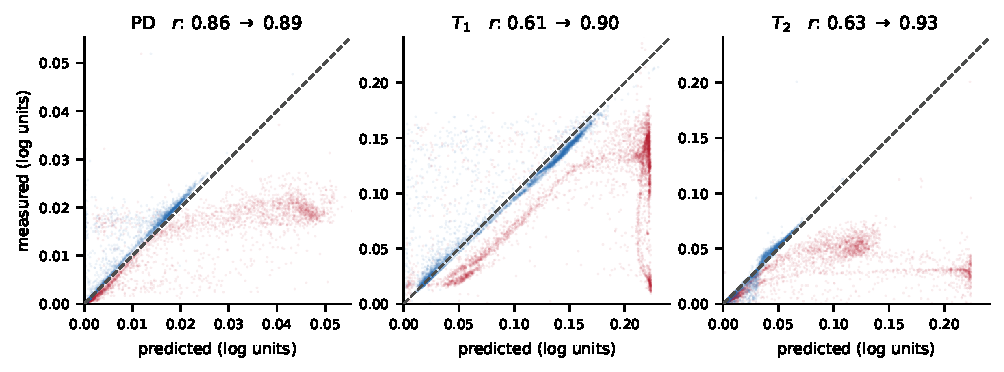
\includegraphics[width=0.56\linewidth]{fig_leak.pdf}
\caption{Measured against predicted displacement, one point per exam. Red is the Fisher
prediction, blue the same with the curvature term restored, dashed is perfect agreement. The red
clouds sit below the line and flatten to the right: for $T_1$, Fisher predicts over $0.95$ of the
full shift on $50.9\%$ of exams. Panel titles give the correlation with the measurement, before
and after \claim{C47}.}
\label{fig:leak}
\end{figure}

\begin{table}[h]\centering\small
\begin{tabular}{lccccc}
\toprule
 & measured & Fisher predicts & measured/predicted & 95\% CI & below pred. \\
\midrule
PD & $+0.003$ & $+0.004$ & $0.706$ & $[0.700,\,0.715]$ & $92.8\%$ \\
$T_1$          & $+0.119$ & $+0.212$ & $0.636$ & $[0.633,\,0.639]$ & $93.9\%$ \\
$T_2$          & $+0.009$ & $+0.017$ & $0.617$ & $[0.607,\,0.626]$ & $98.8\%$ \\
\bottomrule
\end{tabular}
\caption{Distance the estimate moves when the prior's nominal value is raised by $1.25\times$,
in log units, over 4{,}608 exams. The first three columns are medians over exams and do not
divide into one another; the ratio column is the median of per-exam ratios, which is the quantity
under test. Intervals resample patients. \claim{C23}}
\label{tab:main}
\end{table}

The final column is a sign test, immune to the ratio's scale: nearly every exam moves less
than predicted.

\paragraph{Variation across instruments.} Grouped by instrument, the $T_1$
ratio runs $0.582$ to $0.658$ across three hardware generations of one vendor, a spread of
$0.077$. The extremes are two of the largest groups ($n=771$, $n=2075$), not the smallest
\claim{C24}, and PD and $T_2$ separate further. The shortfall is a property of the instrument as
well as the method, so a correction calibrated on one scanner should not be assumed to transfer.

\paragraph{The omitted curvature term.} With more parameters than
measurements the model fits any attainable data exactly, so the residual in
equation~\ref{eq:hessian} measures what the prior's pull leaves behind, and does not
shrink as the noise does. On the median protocol the dropped term is $0.14\%$ of the Fisher matrix norm, but the norm is
the wrong scale: along $v$ the data contributes no curvature, so the comparison is against
$\lambda$, and there $v^\top C v / \lambda = 0.655$. It moves the predicted $T_1$ leak from $0.941$
to $0.547$, the sensitivity derived in Section~2 \claim{C49}. Recomputing with the exact curvature brings all three ratios to within
$6\%$ of $1$: $1.061$, $0.963$ and $1.018$ for PD, $T_1$ and $T_2$ \claim{C20}. The displacement
is differenced one-sidedly at the $1.25\times$ shift, which carries an $O(\Delta)$ error.
Differencing centrally gives $1.011$, $1.012$ and $1.001$ \claim{C109}, so most of what remains
after the correction is the estimator. The two do not chain: $0.941$ and $0.547$ are one protocol's,
the ratios medians over 4{,}608. It holds per exam,
the corrected $T_1$ ratio spanning $0.934$ to $2.3$ across the 5th to 95th percentiles
\claim{C43}. It holds across experiments too: dropping measurements moves the Fisher ratio across $0.147$
and a hundredfold change in prior width across $0.040$, while the corrected ratio spans $0.005$
and $0.007$ \claim{C46}\claim{C45}.

\paragraph{A rank-one correction.} Because the error lives in one
eigendirection, it can be repaired without building $H$: replace $F$'s near-null eigenvalue $f_1$
by $f_1 + v^\top C v$ and leave the rest of the spectrum alone. That directional second derivative
costs two gradient evaluations whatever the parameter count, against $2p$ for a finite-difference
Hessian. On the cohort it reproduces the full-Hessian correction ($1.034$,
$0.960$ and $1.009$ against $1.061$, $0.963$ and $1.018$) and leaves $D$ at $1.000$
\claim{C65}.

%======================================================================
\section{Discussion}

Fisher information answers a design question: what an acquisition can tell you about each
parameter, before any patient is scanned. For that $F$ is exact rather than approximate, follows
from TR, TE and $b$ alone, and is positive semidefinite by construction, while $H$'s residual
arrives only with the images and a completed fit and is indefinite when residuals are large. For
protocol design, $F$ is right and $H$ is unavailable.

The leak matrix asks something else: how far the prior moves the estimate once a parameter
is unidentifiable. Two arguments carry $F$ across that gap. The first is that the
dropped term is proportional to the residuals and vanishes for a perfect fit
\cite[Prop.~2]{kunstner2019}, \cite{transtrum2011} (whose target is the \emph{empirical} Fisher
matrix; with Gaussian noise ours is the true one). It is small, but a small term in a nearly
singular matrix can still have a large effect. The second is that the approximation holds
whenever the model manifold has small curvature \cite{transtrum2012}. That bounds \emph{extrinsic}
curvature, and ours is zero: the Jacobian has full row rank, so the manifold has no normal
direction \claim{C22}. What is left is parameter-effects curvature, removable by a change of
coordinates in general but not here, since the coordinates cannot change without changing the
prior.

\paragraph{Learned estimators.} The leak matrix describes a per-exam optimisation, and an
amortised network never solves one. The direction $v$ survives the change of estimator: it is a
property of the acquisition, and no estimator recovers what three measurements do not determine.
A MAP fit fills that direction from the prior, by the fraction $M_{jj}$. A network's objective
fills it with nothing, so whatever fills it comes from the training run. Self-supervised
physics-guided reconstruction \cite{vanlune2026} minimises the same objective and needs no
reference maps, so this runs on these images. We train five networks differing only in random
seed and split each pair's disagreement on held-out exams along $v$ and across it. Over $80$
exams held out of $292$ the disagreement is $2.28$ times larger along $v$, $0.078$ log units
against $0.034$, with $88.8\%$ of exams following that ordering \claim{C97}; three further
configurations give $3.02$ to $3.19$
\claim{C72}. In the parameter this is an $8.1\%$ difference between two runs of one architecture
on one dataset, the comparison that matches how these methods are deployed. The direction it falls in follows from TR, TE and $b$ before any network is
trained. The comparison is not normalised per dimension and has no matched control, so it carries
the ordering and not the size.

\paragraph{Limitations.} The leak is defined relative to a parametrization. We fit log parameters, in
which the prior is round; fitting $T_1$ and $T_2$ directly, or their inverses $R_1$ and $R_2$,
would give a different prior and a different leak, and we have not measured how much of the
$0.62$ to $0.71$ follows from that choice. Per-voxel noise is unmeasurable on registered clinical
volumes, so $\sigma = 0.05$ is set rather than estimated, though the parameter ordering survives
a $625\times$ sweep of the between-contrast weighting \claim{C8}. All five instruments we compare are one
vendor's \claim{C15}, and unmodelled physics such as magnetization transfer remains a live account
of part of the residual \claim{C16}. A paired cohort on two machines would test the harmonization
claim directly; ours failed its identity control \claim{C12}.

%======================================================================
\section{Conclusion}

The prior's contribution to a fitted MRI parameter is a bias with a closed form. Fisher information
predicts it too large, by 29--38\% over 4{,}608 exams, by amounts that differ across scanners, and
with the exam ordering largely lost. Restoring the discarded curvature term recovers most of it. The measurement
transfers to any underdetermined least-squares fit closed by a prior: take the Fisher matrix's
near-null direction $v$, compare $v^\top C v$ against $\lambda$ rather than against $\|F\|$, and
correct the leak when it is not small. Nothing in that procedure is specific to MRI.

\bibliographystyle{plain}
\begin{thebibliography}{9}
\bibitem{transtrum2011} M.~K. Transtrum, B.~B. Machta, and J.~P. Sethna.
  Geometry of nonlinear least squares with applications to sloppy models and optimization.
  \emph{Physical Review E}, 83:036701, 2011.
\bibitem{transtrum2012} M.~K. Transtrum and J.~P. Sethna.
  Geodesic acceleration and the small-curvature approximation for nonlinear least squares.
  arXiv:1207.4999, 2012.
\bibitem{kunstner2019} F.~Kunstner, L.~Balles, and P.~Hennig.
  Limitations of the empirical Fisher approximation for natural gradient descent.
  \emph{Advances in Neural Information Processing Systems}, 2019.
\bibitem{vallisneri2008} M.~Vallisneri.
  Use and abuse of the Fisher information matrix in the assessment of gravitational-wave
  parameter-estimation prospects. \emph{Physical Review D}, 77:042001, 2008.
\bibitem{borges2023} P.~Borges, V.~Fernandez, P.-D.~Tudosiu, P.~Nachev, S.~Ourselin, and
  M.~J.~Cardoso.
  Unsupervised heteromodal physics-informed representation of MRI data: tackling data
  harmonisation, imputation and domain shift. \emph{SASHIMI, MICCAI Workshops},
  LNCS 14288, 2023.
\bibitem{phycharm2025} G.~Lee, D.~H.~Ye, and S.-H.~Oh. A preliminary attempt to harmonize
  using physics-constrained deep neural networks for multisite and multiscanner MRI datasets
  (PhyCHarm). \emph{NeuroImage}, 317:121361, 2025. doi:10.1016/j.neuroimage.2025.121361.
\bibitem{bloch_pinn2023} Q.~Cai, L.~Zhu, J.~Zhou, C.~Qian, D.~Guo, and X.~Qu.
  Bloch equation enables physics-informed neural network in parametric magnetic resonance
  imaging. arXiv:2309.11763, 2023.
\bibitem{zhang2022} X.~Zhang, Q.~Duchemin, K.~Liu, C.~Gultekin, S.~Flassbeck,
  C.~Fernandez-Granda, and J.~Assl\"ander. Cram\'er--Rao bound-informed training of neural
  networks for quantitative MRI. \emph{Magnetic Resonance in Medicine}, 88(1):436--448, 2022.
\bibitem{vanlune2026} J.~van Lune, S.~Mandija, O.~van der Heide, M.~Maspero, M.~B.~Schilder,
  J.~W.~Dankbaar, C.~A.~T.~van den Berg, and A.~Sbrizzi. Quantitative mapping from conventional
  MRI using
  self-supervised physics-guided deep learning: applications to a large-scale, clinically
  heterogeneous dataset. arXiv:2601.05063, 2026.
\bibitem{qiu2023} H.~Sun, L.~Wang, T.~Daskivich, S.~Qiu, F.~Han, A.~D'Agnolo, R.~Saouaf,
  A.~G.~Christodoulou, H.~Kim, D.~Li, and Y.~Xie. Retrospective T2 quantification from
  conventional weighted MRI of the prostate based on deep learning. 2023. PMC10598780.
\end{thebibliography}
% Read-depth: Transtrum, Kunstner, Vallisneri, Borges, PhyCHarm and van Lune are read in full.
% Zhang 2022 is abstract-only, and is cited for exactly what its abstract states (CRB-normalised
% training loss, verified variance) and nothing more.

\end{document}
